%%%%%%%% HOM dip of quantum-dot photons -- ICML 2026 template %%%%%%%%%%%%%%%%
\documentclass{article}

\usepackage{microtype}
\usepackage{graphicx}
\usepackage{subcaption}
\usepackage{booktabs}
\usepackage{hyperref}
\newcommand{\theHalgorithm}{\arabic{algorithm}}

% preprint option: authors are shown, no "under review" notice
\usepackage[preprint]{icml2026}

\usepackage{amsmath}
\usepackage{amssymb}
\usepackage{mathtools}
\usepackage{amsthm}
\usepackage[capitalize,noabbrev]{cleveref}

\graphicspath{{../results/}}

\newcommand{\Kg}{K_{\mathrm{EG}}}
\newcommand{\Vi}{V_{\mathrm{int}}}
\newcommand{\dd}{\mathrm{d}}
\newcommand{\erfc}{\operatorname{erfc}}

\icmltitlerunning{Anatomy of a Hong--Ou--Mandel dip of quantum-dot photons}

\begin{document}

\twocolumn[
  \icmltitle{Anatomy of a Hong--Ou--Mandel Dip of Quantum-Dot Photons:\\
    Lifetime, Emission-Time Jitter and Coherence from a Single Delay Scan}

  \begin{icmlauthorlist}
    \icmlauthor{Yurii Biriukov}{msu}
  \end{icmlauthorlist}

  \icmlaffiliation{msu}{Quantum Technology Centre, Faculty of Physics,
    Lomonosov Moscow State University, Moscow, Russia}
  \icmlcorrespondingauthor{Yurii Biriukov}{biryukovya@my.msu.ru}

  \icmlkeywords{Hong-Ou-Mandel interference, quantum dot, single photons,
    indistinguishability, model selection}

  \vskip 0.3in
]

\printAffiliationsAndNotice{}

\begin{abstract}
We analyse a Hong--Ou--Mandel (HOM) delay scan of two single photons emitted
by a semiconductor quantum dot $12.1$~ns apart. Starting from the two-time
coherence of a dephased two-level emitter we derive a closed-form dip shape:
an exponential of the radiative lifetime convolved with the distribution of
the photons' emission-time difference. Among seven candidate shapes this
model (and its coherent variant) is the only one that describes the 130 data points at the noise level
(residual rms $1.7\times10^{-3}$, random residuals), whereas the pure
exponential, Lorentzian and Gaussian dips are rejected by $\Delta\mathrm{AICc}>300$.
The fit yields a zero-delay visibility $V_0=0.832\pm0.001_{\rm stat}\pm0.004_{\rm model}$,
a jitter-free interference amplitude $\Vi=0.920\pm0.002$, a radiative
lifetime $T_1=130.8\pm0.7\pm1.9$~ps, an rms emission-time jitter of
$11.9\pm0.3$~ps per photon, a coherence time $T_2\geq 218$~ps and a
homogeneous linewidth $\lesssim 6.0~\mu$eV, $1.2$ times the Fourier limit.
Every number is accompanied by an independent check, and all scripts are
provided.
\end{abstract}

%==============================================================================
\section{Introduction}
\label{sec:intro}

Two-photon interference on a beam splitter \cite{HOM1987} is the standard
benchmark of single-photon sources for linear-optical quantum technologies
\cite{Santori2002,Senellart2017}. When two identical photons meet on a
balanced beam splitter they always leave through the same port, so the
probability of a coincidence between the two outputs vanishes; any
distinguishability in polarisation, spectrum or arrival time restores
coincidences \cite{Branczyk2017}. Scanning the relative delay $\tau$ of the
photons therefore traces a \emph{dip} whose depth measures the photon
indistinguishability and whose \emph{shape} is fixed by the photons'
temporal modes.

Quantum-dot (QD) sources are usually characterised only by the depth of this
dip \cite{Somaschi2016,Ding2016}. The shape, however, contains much more:
the radiative lifetime, the statistics of the emission time, and --- in
combination with the depth --- the coherence time and linewidth of the
emitter. Extracting this information requires (i) a physically motivated
model of the dip and (ii) a careful statistical procedure that shows which
features of the model are actually supported by the data.

In this work we analyse one such delay scan. Our contributions are:
\begin{itemize}
\item A closed-form model of the delay-integrated HOM dip of a dephased
two-level emitter with random emission time (\cref{sec:model}), and an
independent numerical verification of it.
\item A quantitative comparison of seven dip shapes with information criteria,
residual diagnostics, cross-validation and simulation-based power analysis
(\cref{sec:fit}).
\item A full set of source parameters with statistical and model
uncertainties, and an explicit list of the assumptions each one depends on
(\cref{sec:params,sec:verif}).
\end{itemize}

%==============================================================================
\section{Data}
\label{sec:data}

The data set (\texttt{data/data.txt}) contains $n=130$ values of the
normalised coincidence level $C$ between the two outputs of a beam splitter,
recorded as a function of the position $x$ of one of the beam-splitter
inputs, $x=0$--$13.545$~cm in steps of $0.105$~cm (\cref{fig:main}). The two
photons are emitted by the same QD $12.1$~ns apart (consecutive excitation
pulses) and are brought to temporal overlap by a delay line; $x$ fine-tunes
the remaining delay. No error bars, count rates or auxiliary measurements
($g^{(2)}(0)$, beam-splitter ratio, lifetime) are given.

\paragraph{Delay scale.} Moving the input by $\Delta x$ changes the optical path
by $\Delta x$, i.e.\
$\tau = n_g \Delta x/c$ with the group index of air $n_g=1.00028$
($1~\mathrm{cm}\leftrightarrow 33.36$~ps).

\paragraph{Noise level.} A model-free estimate of white noise from second
differences, $\hat\sigma^2 = \langle(y_{i+1}-2y_i+y_{i-1})^2\rangle/6$, gives
$\hat\sigma=1.45\times10^{-3}$; this is the benchmark a correct model must
reach.

%==============================================================================
\section{Model of the dip}
\label{sec:model}

\paragraph{HOM with mixed photons.} For photons $a$ and $b$ with normalised
two-time coherences $G_{a,b}(t,t')=\langle \hat a^\dagger(t)\hat a(t')\rangle$
incident on a beam splitter with reflectivity $R$ and transmissivity $T=1-R$,
the delay-integrated coincidence probability is
\cite{Bylander2003,Kiraz2004,Branczyk2017}
\begin{align}
  P_c(\tau) &= R^2+T^2 - 2RT\,J(\tau), \label{eq:pc}\\
  J(\tau) &= \iint G_a(t,t')\,G_b(t'\!-\!\tau,t\!-\!\tau)\,\dd t\,\dd t'. \nonumber
\end{align}
$J$ is the overlap $\mathrm{Tr}\,\rho_a\rho_b$ of the (in general mixed)
single-photon states; it is bilinear in the states, so classical mixtures
(e.g.\ random emission times) enter as averages of $G$.

\paragraph{Dephased two-level emitter.} A QD excited at $t_0$ and
decaying with rate $\Gamma=1/T_1$ under pure dephasing $\gamma^*$ emits a
photon with
$G(t,t') = \Gamma e^{-\Gamma(t+t'-2t_0)/2}\,e^{-\gamma^*|t-t'|}$ for
$t,t'>t_0$. Inserting it into \cref{eq:pc} gives (\cref{app:deriv})
\begin{equation}
  J(\tau) = \frac{T_2}{2T_1}\,e^{-|\tau|/T_1},\qquad
  \frac{1}{T_2}=\frac{1}{2T_1}+\gamma^* .
  \label{eq:exp}
\end{equation}
Dephasing lowers the depth but not the shape; a slowly wandering central
frequency (constant within one photon) likewise only lowers the depth, since
$|\langle\psi_a|\psi_b\rangle|^2 = e^{-|\tau|/T_1}/(1+\delta^2T_1^2)$ for a
detuning $\delta$. Detector timing jitter is irrelevant for
delay-integrated coincidences.

\paragraph{Emission-time jitter.} Under pulsed excitation the photon does not
start at a fixed time: relaxation from higher states, phonon-assisted
processes or a finite pulse length randomise $t_0$
\cite{Kiraz2004,Unsleber2015}. Averaging \cref{eq:exp} over the
distribution of $\Delta t_0=t_{0a}-t_{0b}$ convolves the exponential with that
distribution. For Gaussian jitter of rms $\sigma_1$ per photon
($\Delta t_0$ Gaussian with $s=\sqrt2\sigma_1$), with $L=cT_1$ and $u=|x-x_0|$,
\begin{align}
  \Kg(u) &= \tfrac12 e^{s^2/2L^2}\Big[e^{-u/L}\erfc\tfrac{s/L-u/s}{\sqrt2}
             \nonumber\\ &\qquad\qquad
             + e^{u/L}\erfc\tfrac{s/L+u/s}{\sqrt2}\Big],
  \label{eq:keg}
\end{align}
which rounds the cusp of the exponential and reduces the zero-delay overlap
to $\Kg(0)=e^{s^2/2L^2}\erfc(s/\sqrt2L)<1$. For exponential feeding with
time constant $l_r$, $\Delta t_0$ is Laplace-distributed and
$K_{\mathrm{EL}}(u)=\frac{b}{b^2-a^2}(b e^{-au}-a e^{-bu})$, $a=1/L$, $b=1/l_r$.

\paragraph{Fit function.} Collecting all depth-reducing effects in one
amplitude, the model is
\begin{equation}
  C(x) = A\,\big[1 - \Vi\,\Kg(x-x_0;\,L,s)\big],
  \label{eq:model}
\end{equation}
with five parameters: the level $A$ for distinguishable photons, the
jitter-free amplitude $\Vi$, the zero-delay position $x_0$, the lifetime
length $L$ and the jitter width $s$. The observable visibility at zero
delay is $V_0=\Vi\Kg(0)=1-C(x_0)/A$. For a balanced beam splitter and
$g^{(2)}(0)=0$, $\Vi=T_2/2T_1$.

\paragraph{Alternatives.} We also fit (i) a \emph{coherent} variant in which
the jitter is replaced by a pure wave packet $\psi=g\ast e^{-t/2T_1}$ shaped by
a Gaussian pulse $g$ (then $J=[\,K_{\rm EG}(u;2L,s)/K_{\rm EG}(0;2L,s)]^2$
and the amplitude equals $V_0$ directly); (ii) the pure exponential
\cref{eq:exp}; (iii) Laplace jitter; (iv) Gaussian and (v) Lorentzian dips
(expected for Gaussian or exponential spectra, e.g.\ filtered parametric
sources \cite{Branczyk2017}); (vi) an asymmetric variant with separate $L$ on
the two sides of $x_0$, as a symmetry test.

%==============================================================================
\section{Fitting and model selection}
\label{sec:fit}

All models are fitted by unweighted least squares (Levenberg--Marquardt).
We compare them with the corrected Akaike criterion AICc and BIC
\cite{Burnham2002}, and test the residuals with the Wald--Wolfowitz runs
test, the Durbin--Watson statistic (DW; 2 for uncorrelated residuals) and the
Shapiro--Wilk normality test. Uncertainties are 68\% intervals from 3000
residual-bootstrap and 1000 moving-block-bootstrap replicas (block length
8) \cite{Efron1993}.

\begin{figure}[t]
  \centering
  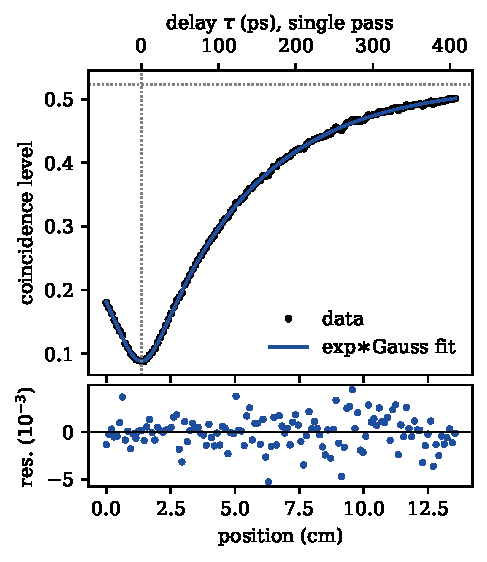
\includegraphics[width=\columnwidth]{fig_fit_main.pdf}
  \caption{Coincidence level versus input position (dots) and the fit of the
  exponential$\ast$Gaussian model, \cref{eq:model} (line). Dotted lines: $A$
  and $x_0$. Top axis: delay for $p=1$. Bottom: residuals, rms
  $1.69\times10^{-3}$.}
  \label{fig:main}
\end{figure}

\begin{table}[t]
  \caption{Model comparison ($n=130$). $\sigma$: residual rms;
  runs: observed/expected number of sign runs; $p_{\rm runs}$: two-sided
  runs-test $p$-value; DW: Durbin--Watson; CV: 10-fold cross-validated rms
  prediction error for random / contiguous folds (in $10^{-3}$).}
  \label{tab:models}
  \vskip 0.05in
  \centering
  \small
  \setlength{\tabcolsep}{3pt}
  \begin{tabular}{lcccccc}
    \toprule
    model & $k$ & $10^3\sigma$ & $\Delta$AICc & runs & DW & CV \\
    \midrule
    exp$\ast$Gauss & 5 & 1.69 & 0.1   & 59/66 & 1.65 & 1.70/1.99 \\
    coherent       & 5 & 1.69 & 0     & 61/66 & 1.65 & 1.70/1.96 \\
    exp$\ast$Laplace & 5 & 1.75 & 8.6 & 58/65 & 1.56 & 1.78/4.02 \\
    asymmetric     & 6 & 1.70 & 2.0   & 57/66 & 1.66 & -- \\
    exponential    & 4 & 5.41 & 301   & 27/66 & 0.30 & 5.69/12.5 \\
    Lorentzian     & 4 & 8.04 & 404   & 13/66 & 0.10 & 8.26/31.5 \\
    Gaussian       & 4 & 16.7 & 594   & 5/66  & 0.04 & 17.4/53.3 \\
    \bottomrule
  \end{tabular}
\end{table}

\paragraph{Results.} \Cref{tab:models} and \cref{fig:resid} summarise the
comparison. The Gaussian and Lorentzian shapes leave oscillating residuals of
$\pm20$--$50\times10^{-3}$ and are rejected: the dip has exponential wings, as
expected for spontaneous emission (Lorentzian spectrum). The pure
exponential describes the wings but not the bottom of the dip, which is
rounded over $\approx\!\pm0.5$~cm (\cref{fig:zoom}); the residuals are
strongly correlated (DW $=0.30$, $p_{\rm runs}=6\times10^{-12}$). Adding
Gaussian emission-time jitter reduces the residual rms by a factor of 3.2,
to within 17\% of the model-free noise estimate, and makes the residuals
compatible with white Gaussian noise ($p_{\rm runs}=0.23$, Shapiro--Wilk
$p=0.31$; the mild DW $=1.65$ is covered by the block bootstrap).

\paragraph{Shape of the jitter.} Gaussian jitter is preferred over
exponential (Laplace) jitter by $\Delta\mathrm{AICc}=8.5$, and the Laplace
model fails markedly in contiguous cross-validation (4.0 vs
$2.0\times10^{-3}$), because it predicts a too-deep minimum
($C_{\min}=0.0857$ vs.\ $0.0878$). To check that this preference is not a
statistical fluctuation we simulated 300 data sets from the best Laplace
model with the observed noise: the Gaussian model was preferred in only 7 of
them, and never by as much as observed ($p<0.003$).

\paragraph{Coherent vs.\ incoherent.} The coherent pulse-shaped wave packet
and the incoherent Gaussian jitter give numerically indistinguishable shapes
($\Delta\mathrm{AICc}=0.1$): as long as the jitter is much shorter than $T_1$
both reduce to an exponential with a rounded tip. The data therefore fix the
width of the rounding, but not whether it is coherent. This ambiguity matters
only for the interpretation of $\Vi$, not for $V_0$, which is identical in
both models (\cref{tab:params}).

\paragraph{Symmetry.} Fitting separate decay lengths left and right of the
minimum gives $L_1=4.00\pm0.14$~cm and $L_2=3.92\pm0.02$~cm, consistent
with a symmetric dip; the extra parameter is not supported
($\Delta\mathrm{AICc}=+2.0$).

\begin{figure}[t]
  \centering
  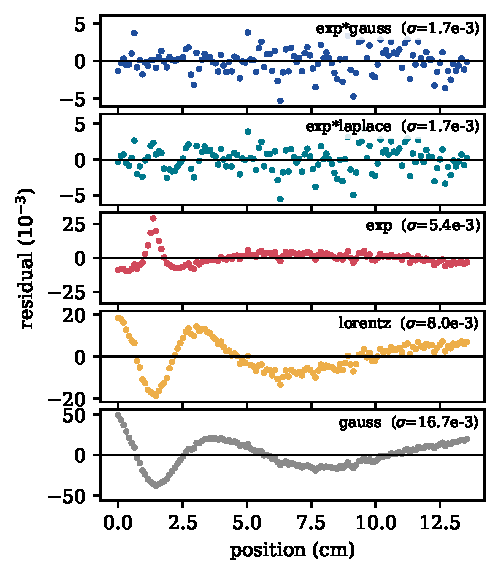
\includegraphics[width=\columnwidth]{fig_residuals_models.pdf}
  \caption{Residuals of five dip models (note the different vertical scales).
  Only the models with emission-time jitter give structureless residuals.}
  \label{fig:resid}
\end{figure}

\begin{figure}[t]
  \centering
  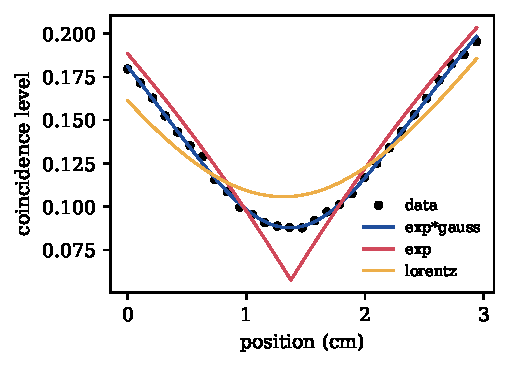
\includegraphics[width=0.85\columnwidth]{fig_zoom.pdf}
  \caption{Bottom of the dip. The pure exponential has a cusp at $x_0$ that
  the data do not show; the Lorentzian is too flat. The rounding is
  reproduced by an emission-time jitter of $\sigma_1\approx12$~ps.}
  \label{fig:zoom}
\end{figure}

%==============================================================================
\section{Physical parameters}
\label{sec:params}

\begin{table}[t]
  \caption{Parameters of the exp$\ast$Gauss model and derived quantities.
  Errors: residual bootstrap (block bootstrap agrees within 10\%); where
  given, the second error is the spread among the three acceptable models
  (exp$\ast$Gauss, coherent, exp$\ast$Laplace). $V_0$: zero-delay visibility;
  $\Vi$: jitter-free amplitude; $\Kg(0)$: jitter-limited overlap;
  $\sigma_1$: rms emission-time jitter per photon; $T_2^*=1/\gamma^*$;
  $\Delta\nu=1/\pi T_2$; $1/2\pi T_1$: Fourier limit; $cT_2$: coherence
  length. Pairs ``a / b'' are obtained from $V_0$ / $\Vi$.}
  \label{tab:params}
  \vskip 0.05in
  \centering
  \footnotesize
  \setlength{\tabcolsep}{2pt}
  \begin{tabular}{lc}
    \toprule
    quantity & value \\
    \midrule
    $A$ (distinguishable level) & $0.5231\pm0.0006$ \\
    $x_0$ (cm) & $1.366\pm0.004\pm0.004$ \\
    $V_0$ & $0.8321\pm0.0012\pm0.004$ \\
    $\Vi$ & $0.9196\pm0.0015$ \\
    $\Kg(0)$ & $0.905\pm0.002$ \\
    $L$ (cm) & $3.921\pm0.020$ \\
    $s$ (cm) & $0.506\pm0.011$ \\
    dip FWHM (cm) & $6.28\pm0.02$ \\
    \midrule
    $T_1$ (ps) & $130.8\pm0.7\pm1.9$ \\
    jitter $\sigma_1$ (ps) & $11.9\pm0.3$ \\
    dip FWHM (ps) & $209.7\pm0.7$ \\
    $T_2$ (ps) & $218$ / $241$ \\
    $T_2^*$ (ns) & $1.30$ / $2.99$ \\
    $\Delta\nu$ (GHz) & $1.46$ / $1.32$ \\
    $\hbar\Delta\omega$ ($\mu$eV) & $6.05$ / $5.47$ \\
    $1/2\pi T_1$ (GHz) & $1.217$ \\
    $cT_2$ (cm) & $6.5$ / $7.2$ \\
    \bottomrule
  \end{tabular}
\end{table}

\Cref{tab:params} lists the results. We discuss them in order of decreasing
robustness.

\paragraph{Zero-delay visibility.} $V_0=0.832$ is the most robust number: it
is identical in the incoherent and coherent models, changes by at most
$0.004$ for Laplace jitter, and a model-light estimate (parabola through the
seven lowest points, $C_{\min}=0.08788$, with $A$ from a tail-only fit)
gives $0.831$. For a balanced beam splitter, perfect mode matching and
$g^{(2)}(0)=0$ it equals the two-photon indistinguishability $M$; all
experimental imperfections lower the visibility, so $M\ge V_0$. With the
correction of \citet{Ollivier2021},
$M=(V_0+g^{(2)})/(1-g^{(2)})$, one would obtain $M=0.851$, $0.869$ and
$0.929$ for $g^{(2)}(0)=0.01$, $0.02$ and $0.05$.

\paragraph{Lifetime.} The exponential wings fix $L=3.92$~cm, i.e.\
$T_1=131$~ps, a Purcell-shortened lifetime typical of QDs in micropillar
cavities \cite{Somaschi2016,Ding2016}. The value is stable to $0.5\%$ on all
subsets of the data (\cref{app:subsets}) and changes by $1.5\%$ between the
acceptable models. The single-photon wave packet is $cT_1=3.9$~cm long.

\paragraph{Emission-time jitter.} The rounding of the tip corresponds to an
rms jitter of $\Delta t_0$ of $16.9\pm0.4$~ps, i.e.\ $\sigma_1=11.9\pm0.3$~ps
per photon (Laplace model: feeding time $14$~ps; coherent model: pulse
intensity rms $8.6$~ps). Such values are typical of excitation pulses of
several ps or of phonon-assisted/relaxation-based excitation
\cite{Unsleber2015,IlesSmith2017}. The jitter alone limits the overlap to
$\Kg(0)=0.905$: if it is incoherent, it accounts for about half of the total
visibility loss $1-V_0$.

\paragraph{Coherence time and linewidth.} Because $\Vi\le T_2/2T_1$ (equality
for a balanced beam splitter and $g^{(2)}=0$), the dip yields a
\emph{lower} bound on $T_2$: $T_2\ge 2\Vi T_1=241$~ps if the jitter is
incoherent, or $T_2\ge 2V_0T_1=218$~ps in the most conservative case. The
homogeneous linewidth is correspondingly at most $1.46$~GHz ($6.0~\mu$eV),
only $1.1$--$1.2$ times the Fourier limit of $1.22$~GHz ($5.0~\mu$eV); the
pure-dephasing time is $T_2^*\ge1.3$~ns. Since the two photons are
separated by $12.1$~ns, spectral wandering slower than this does not enter;
the numbers characterise dephasing on the $\lesssim\!10$~ns scale.

\paragraph{Normalisation.} The asymptote $A=0.523$ exceeds the value $1/2$
expected for distinguishable photons on a balanced beam splitter, and
forcing $A=1/2$ is excluded (the last points already exceed $0.50$; even a
bi-exponential kernel then gives $\sigma=6.3\times10^{-3}$). If $C$ were an
absolute probability, \cref{eq:pc} would imply $R^2+T^2=A$, i.e.\
$R\approx0.39$, and a maximal visibility $2RT/(R^2+T^2)=0.912$. This is
compatible with $V_0$ (giving a corrected $M\approx0.913$), but is violated
by $\Vi=0.920$ at $4.2\sigma$. Thus either the data are normalised to an
arbitrary reference, or the jitter is (at least partly) coherent; the
present data cannot decide. Also, if $\Vi$ were the true $M$, positivity of
$1-M$ would bound $g^{(2)}(0)\le(1-\Vi)/2=0.040$.

\paragraph{Zero delay.} The overlap position $x_0=1.366$~cm marks where the
delay line compensates the $12.1$~ns separation exactly (an unfolded path of
$c\cdot12.1~\mathrm{ns}=3.63$~m in air). It is determined to $\pm40~\mu$m,
i.e.\ $\pm0.13$~ps.

%==============================================================================
\section{Verification}
\label{sec:verif}

Each claim above was checked independently of the fit that produced it
(scripts in \texttt{src/}, logs in \texttt{results/}):

\begin{enumerate}
\item \textbf{Analytic kernel.} $J(\tau)$ was computed by brute-force
double integration of $G_a G_b$ on a time grid (\texttt{verify\_model.py}),
for $T_1=130$~ps, $T_2^*=3$~ns, $\sigma_1=12$~ps, without using
\cref{eq:exp,eq:keg}. The relative deviation from $\frac{T_2}{2T_1}\Kg$ is
$2.5\times10^{-3}$ at a 1~ps grid and $1.3\times10^{-3}$ at 0.5~ps, i.e.\ it
vanishes linearly with the step. The coherent-model formula agrees to
$<10^{-4}$. The closed form \cref{eq:keg} also agrees with direct quadrature
of the convolution to better than $10^{-15}$.
\item \textbf{Global minimum.} Differential evolution over wide bounds
reproduces the Levenberg--Marquardt parameters to $<4\times10^{-8}$.
\item \textbf{Error bars.} In 400 injection--recovery simulations the fit is
unbiased ($|\mathrm{bias}|<0.1\sigma$) and the covariance errors have
65--69\% coverage; residual- and block-bootstrap errors agree within 10\%. A
fit weighted with Poisson-like errors $\propto\sqrt{C}$ changes $\Vi$, $L$
and $s$ by less than $1\sigma$.
\item \textbf{Model selection.} AICc, BIC and cross-validation give the same
ranking; the Gauss-vs-Laplace preference was tested by simulation
(\cref{sec:fit}).
\item \textbf{Robustness.} Fits to subsets (only $x\le9$~cm, $x\ge0.5$~cm,
without the minimum, even or odd points) agree within $1\sigma$
(\cref{app:subsets}).
\item \textbf{Visibility.} Model-light estimate of $V_0$ ($0.831$) agrees
with the model ($0.832$).
\end{enumerate}

%==============================================================================
\section{Limitations}

The beam-splitter ratio, $g^{(2)}(0)$, polarisation and spatial mode overlap
are not known, so $V_0$ and $\Vi$ only bound $M$ and $T_2$ from below. The
model assumes identical photons from the two pulses (same $T_1$ and
spectrum). The noise model is empirical: without raw counts we cannot test
Poisson statistics directly. An independent time-resolved lifetime
measurement would test $T_1$; a $g^{(2)}$ measurement and a scan with
orthogonal polarisations (which gives $A$ directly) would convert the bounds
on $M$ and $T_2$ into values.

%==============================================================================
\section{Conclusion}

A single HOM delay scan of QD photons contains far more than a visibility.
The dip is exponential in its wings, with a rounded tip; a two-level
emitter with dephasing and $\approx12$~ps Gaussian emission-time jitter
reproduces all 130 points at the noise level. From the fit we obtain the
lifetime ($131$~ps), the jitter, the zero-delay visibility ($0.832$), a
jitter-free amplitude ($0.920$), and lower bounds on the coherence time
($\ge218$~ps) and on how close the photons are to the Fourier limit
(within a factor $1.2$). The main systematic uncertainty is the delay scale,
which can be removed by a single auxiliary measurement.

\section*{Software and Data}
The analysis code is in \texttt{src/} (models, fits, verification) and its
output in \texttt{results/}; the raw data in \texttt{data/data.txt} were
not modified. \texttt{python src/fit\_hom.py} reproduces all tables and
figures.

\section*{Impact Statement}
This paper presents work whose goal is to advance the characterisation of
single-photon sources for quantum technologies. There are many potential
societal consequences of our work, none which we feel must be specifically
highlighted here.

\bibliography{hom_dip}
\bibliographystyle{icml2026}

%==============================================================================
\newpage
\appendix
\onecolumn

\section{Derivation of the kernel}
\label{app:deriv}

With $G(t,t')=\Gamma e^{-\Gamma(t+t')/2}e^{-\gamma^*|t-t'|}\theta(t)\theta(t')$
for photon $a$ and the same function shifted by $\tau>0$ for photon $b$,
\begin{align*}
J(\tau) &= \Gamma^2\iint_{t,t'>\tau} e^{-\Gamma(t+t')/2}\,
          e^{-\Gamma(t+t'-2\tau)/2}\, e^{-2\gamma^*|t-t'|}\,\dd t\,\dd t'
        = \Gamma^2 e^{-\Gamma\tau}\iint_{u,u'>0}
          e^{-\Gamma(u+u')}e^{-2\gamma^*|u-u'|}\,\dd u\,\dd u' \\
        &= 2\Gamma^2 e^{-\Gamma\tau}\int_0^\infty e^{-2\Gamma u}\,\dd u
          \int_0^\infty e^{-(\Gamma+2\gamma^*)v}\,\dd v
        = \frac{\Gamma}{\Gamma+2\gamma^*}\,e^{-\Gamma\tau}
        = \frac{T_2}{2T_1}\,e^{-|\tau|/T_1},
\end{align*}
using $u=t-\tau$, $v=u'-u$ and $1/T_2=\Gamma/2+\gamma^*$; $\tau<0$ follows by
symmetry. With random start times, $G\to\langle G_{t_0}\rangle$; since $J$ is
bilinear and depends only on $\tau+t_{0a}-t_{0b}$, it becomes the
convolution of \cref{eq:exp} with the probability density of
$\Delta t_0=t_{0a}-t_{0b}$. For $\Delta t_0\sim\mathcal N(0,s^2)$,
$\int e^{-|u-w|/L}\,\mathcal N(w;0,s^2)\,\dd w$ evaluates to \cref{eq:keg}
by splitting the integral at $w=u$ and completing the square. For a
coherent pulse, $\psi = g\ast\phi$ with $\phi(t)=\sqrt\Gamma
e^{-\Gamma t/2}\theta(t)$ and the overlap amplitude is the autocorrelation
$(g\star g)\ast(\phi\star\phi)$; for a Gaussian $|g|^2$ of rms $\sigma_p$,
$g\star g$ is Gaussian with $s=2\sigma_p$ and $\phi\star\phi=e^{-|\tau|/2T_1}$,
which gives the coherent model of \cref{sec:model}.

\section{Parameter stability and bootstrap distributions}
\label{app:subsets}

\begin{table}[h]
  \caption{exp$\ast$Gauss fits on subsets of the data (errors from the
  covariance matrix).}
  \vskip 0.05in
  \centering
  \small
  \begin{tabular}{lccccc}
    \toprule
    subset & $A$ & $\Vi$ & $x_0$ (cm) & $L$ (cm) & $s$ (cm) \\
    \midrule
    all points           & 0.5231(6)  & 0.9196(15) & 1.3662(41) & 3.921(20) & 0.506(11) \\
    $x\le 9$ cm          & 0.5236(19) & 0.9187(18) & 1.3655(38) & 3.938(41) & 0.501(12) \\
    $x\ge 0.5$ cm        & 0.5231(7)  & 0.9186(19) & 1.3700(58) & 3.922(21) & 0.498(14) \\
    without $|x-x_0|<0.3$ cm & 0.5230(7) & 0.9197(16) & 1.3662(42) & 3.919(21) & 0.509(16) \\
    even points          & 0.5228(8)  & 0.9196(20) & 1.3687(51) & 3.911(26) & 0.508(15) \\
    odd points           & 0.5233(10) & 0.9196(24) & 1.3635(65) & 3.930(32) & 0.504(18) \\
    \bottomrule
  \end{tabular}
\end{table}

The correlation coefficients of the main fit are largest between $A$ and $L$
($+0.91$), $\Vi$ and $L$ ($-0.79$), and $\Vi$ and $s$ ($+0.78$): a longer
lifetime is partly traded against a higher asymptote, and a deeper intrinsic
dip against a wider jitter. The bootstrap distributions
(\cref{fig:boot}) are unimodal and nearly Gaussian.

\begin{figure}[h]
  \centering
  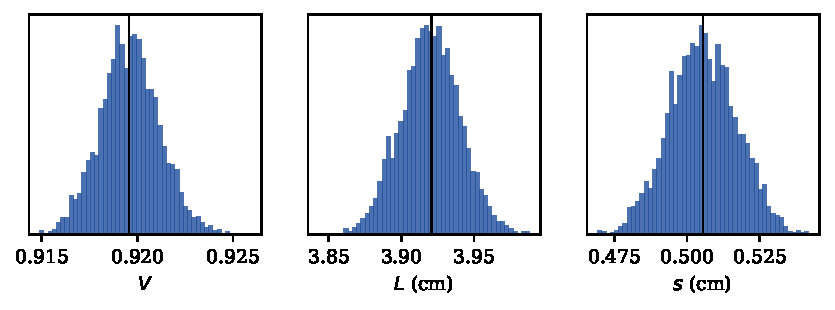
\includegraphics[width=0.8\textwidth]{fig_bootstrap.pdf}
  \caption{Residual-bootstrap distributions (3000 replicas) of $\Vi$, $L$ and
  $s$; vertical lines: best fit.}
  \label{fig:boot}
\end{figure}

\end{document}
